For continuous data, two mapping techniques are commonly used: choropleth and isarithmic mapping. This chapter will only cover choropleth mapping because the practical part of this thesis will not feature isarithmic mapping. The basic idea of choropleth mapping is applying value or color intensity based on some statistical value to enumeration units like census tracts, counties, states or nations. The higher a value assigned to an enumeration unit, the more saturated the color of that unit. Fundamental to this type of mapping is standardization and classification of raw data. If this is not the case and raw data is used, the visualization will suffer from an inherent areal bias \iacite{McMaster2010}. This problem is best described with a practical example: the united kingdom has higher population but less area compared to canada. However, if the mapped data is not standardized by area, canada will have a higher visual impact than united kingdom due to their superior areal extent, even though the attribute mapped onto canada has a lower value compared to the one on united kingdom. Therefore the less the mapped attribute is tied to enumeration units, the less sense a choropleth map makes.

The following list shows the most rudimentary and most common methods to classify data mentioned by \citeauthor{McMaster2010}. The amount of classes must be known before and to explain the classifications below, five different classes with a value range from 10 to 85 is used. Figure \ref{fig:choropleth-classification} on page \pageref{fig:choropleth-classification} illustrates an example showing all values as circles on the top and their corresponding classification downwards.

\begin{figure}[!htb]
\centering
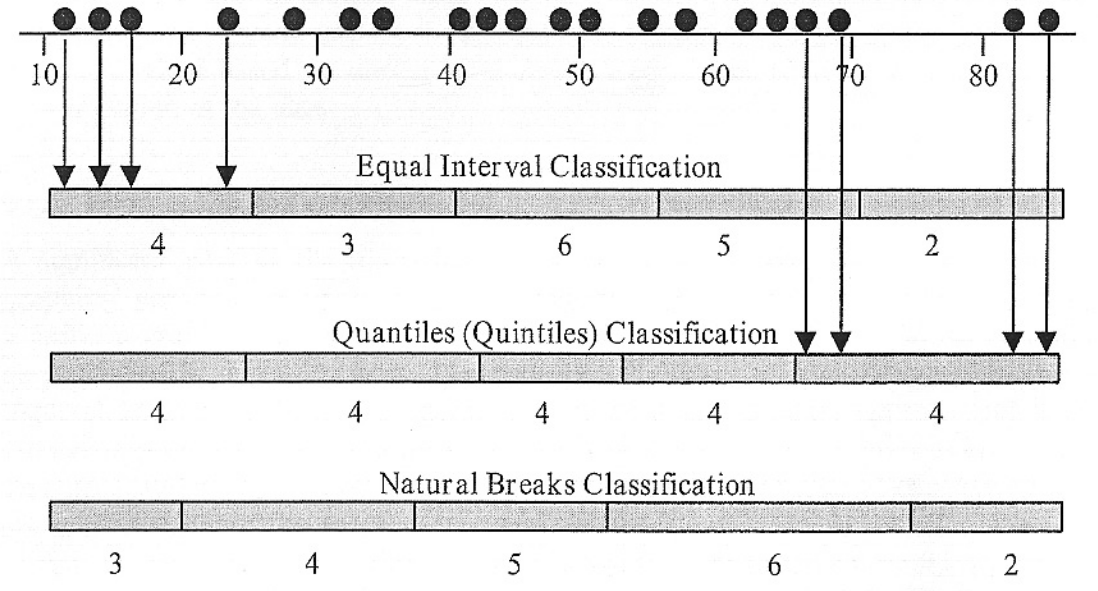
\includegraphics[height=5cm,keepaspectratio]{images/choropleth/classification.png}
\caption[
    Data classification techniques \iacite{McMaster2010}.
]{Data classification techniques}
\label{fig:choropleth-classification}
\end{figure}

\begin{itemize}

\item \textbf{Equal interval classification} assumes equal range between the class breaks. With the mentioned example, class one would include values from 10 to 25, class two would include values from 25 to 40, and so forth \iacite{McMaster2010}.

\item \textbf{Quantiles classification} needs to know the amount of items in a dataset in addition to the amount of desired classes. Consider 100 observations in a dataset and five desired classes. Thus, 20 observations will be placed in each class. These 20 observations can be thought of as data values. Putting this amount of data values in five different classes results in 4 data values per class. Now it is only needed to go through the whole dataset and put the first to the fourth item in the first class, the fifth to the ninth item in the second class, and so forth \iacite{McMaster2010}.

\item \textbf{Natural breaks classification} follows the idea of minimizing the internal variation of the dataset, while maximizing the variation among the classes. The user needs to choose significant gaps in the dataset, according to the number of desired classes \iacite{McMaster2010}.

\end{itemize}

In order to create meaninful choropleth maps, some design principles need to be considered:

\begin{itemize}

\item The visual channel this type of mapping is based on should always be a sequential or diverging color scheme for continuous data, depending on wheter there is a meaningful zero point or not. Figure \ref{fig:colorbrewer} on page \pageref{fig:colorbrewer} shows three different categories of color scales. The reason why choropleth maps should only use diverging or sequential sacles is the perception. These two types are always preceived as ordered. Due to their brightness and saturation, they can be ordered from low to high or vice versa, whereas qualitative scales are perceptually nonlinear. Those scales are best used for categorical data.

\item Choropleth maps are commonly used with data representing derived quantities. Examples of derived quantities are density, average, rate and percentage. If this type of map is not used with such data, it has to be read with caution. Aggregated data e.g. crimes committed or amount of orders can also be used, if the areal bias is taken into consideration when interpreting the map.

\item A choropleth map without a legend is not negotiable, according to \citeauthor{Dent2008}. All colors on the map represent a specific value or class, which is defined and explained in the legend. All classifications would be pointless without a map legend \iacite{Dent2008}.

\end{itemize}

\begin{figure}[!htb]
\centering
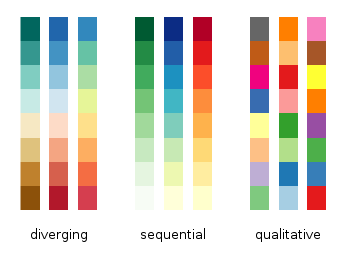
\includegraphics[height=5cm,keepaspectratio]{images/choropleth/color-scales.png}
\caption[
    Three different categories of color scales, Urldate: 07.2016 \newline
    \small\texttt{\url{http://www.gnuplotting.org/figs/colorbrewer.png}}
]{Three different categories of color scales.}
\label{fig:colorbrewer}
\end{figure}

Until now, only so called classed choropleth maps were decribed. Unclassed choropleth maps follow the idea of "letting the data speak for itself". This specific type of a choropleth map assigns a unique color to each unique data value without previous classification. They also make use of a continuous color scale. The major difference to classed ones is best described with an example: consider a dataset consisting of unemployment rates for each state in the united states. If there is a big numerical gap between the second and third highest unemployment rate for two states, their corresponding color would also have a significant jump. Thus the data is placed proportionally along the color scale. Figure \ref{fig:classed-unclassed-choropleth} on page \pageref{fig:classed-unclassed-choropleth} features an unclassed and classed choropleth map.

\begin{figure}[!htb]
  \captionsetup[subfigure]{justification=centering}
  \centering
  \begin{subfigure}[b]{0.4\textwidth}
    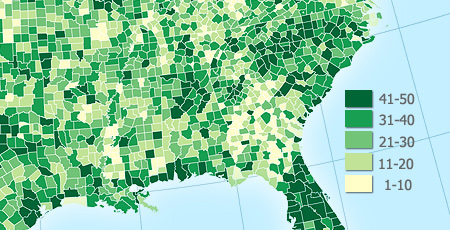
\includegraphics[width=\textwidth]{images/choropleth/classed.jpg}
    \caption{Diverging x diverging bivariate color scale.}
  \end{subfigure}
  \hfill
  \begin{subfigure}[b]{0.4\textwidth}
    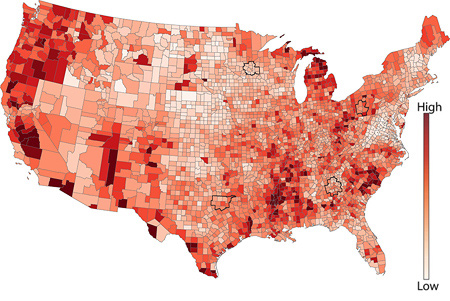
\includegraphics[width=\textwidth]{images/choropleth/unclassed.jpg}
    \caption{Sequential x sequential bivariate color scale.}
  \end{subfigure}
  \caption[
    Comparison of an unclassed and classed choropleth map, Urldate: 07.2016 \newline
    \small\texttt{\url{http://indiemapper.com/app/learnmore.php?l=choropleth}}
  ]{
    Comparison of an unclassed and classed choropleth map.
  }
  \label{fig:classed-unclassed-choropleth}
\end{figure}

The main objective of choropleth maps is to depict the geographic distribution of the data magnitudes. Ideally the choice of fill will communicate the range from low data magnitudes to high magnitudes through an obvious change from light to dark. If an overall geographic pattern should be shown in the map, an unclassed choropleth map is the way to go. If that is not the case and locations should be comparable against each other, classed choropleth maps should be used.


